\documentclass[11pt,a4paper]{article}
\usepackage{TeX_definitions}
\geometry{left=2.4cm,right=2.4cm,top=2.4cm,bottom=2.4cm}
\graphicspath{{figures/}}
\hypersetup{colorlinks=true,linkcolor=blue,citecolor=blue,urlcolor=blue}

\title{Analysis 4-2: family separability on the existing stimulus library}
\author{}
\date{\today}
\begin{document}
\maketitle

\section{Question}
Analysis 4-2 asks whether the rooted-shell library inherited from analyses 2 and 3 already separates the candidate families defined in Analysis 4-1. The target of comparison remains the family-specific belief over the queried node.

\section{Method}
Standard graphical-model background and notation are treated in the usual way; see \cite{Koller2009}.


We evaluated the six canonical families on 600 rooted graph/evidence conditions. For each condition we computed family posteriors, pairwise Jensen--Shannon divergences, a noisy synthetic recovery matrix, descriptor-conditioned summaries, and a reduced stimulus panel.

\section{Results}
The full library produces a clear hierarchy. The strongest average family contrast is between $M_{\mathrm{exact}}$ and $M_{\mathrm{star}}$ (mean JS 0.113605), followed by $M_{\mathrm{star}}$ and $M_{\mathrm{cluster}}$ (mean JS 0.10413). By contrast, canonical $M_{\rho}$ stays close to $M_{\mathrm{exact}}$ on the current library (mean JS 0.009751), showing that the present task family is better at separating structure rewrites from exact inference than at isolating subtle attenuation on the true graph.

The reduced panel retained six high-value conditions: RG119 (high), RG112 (high), RG121 (high), RG114 (high), RG036 (high), RG100 (high). These conditions cover all three D3 classes and provide the basis for later identifiability and design analyses.

\begin{figure}[H]
\centering
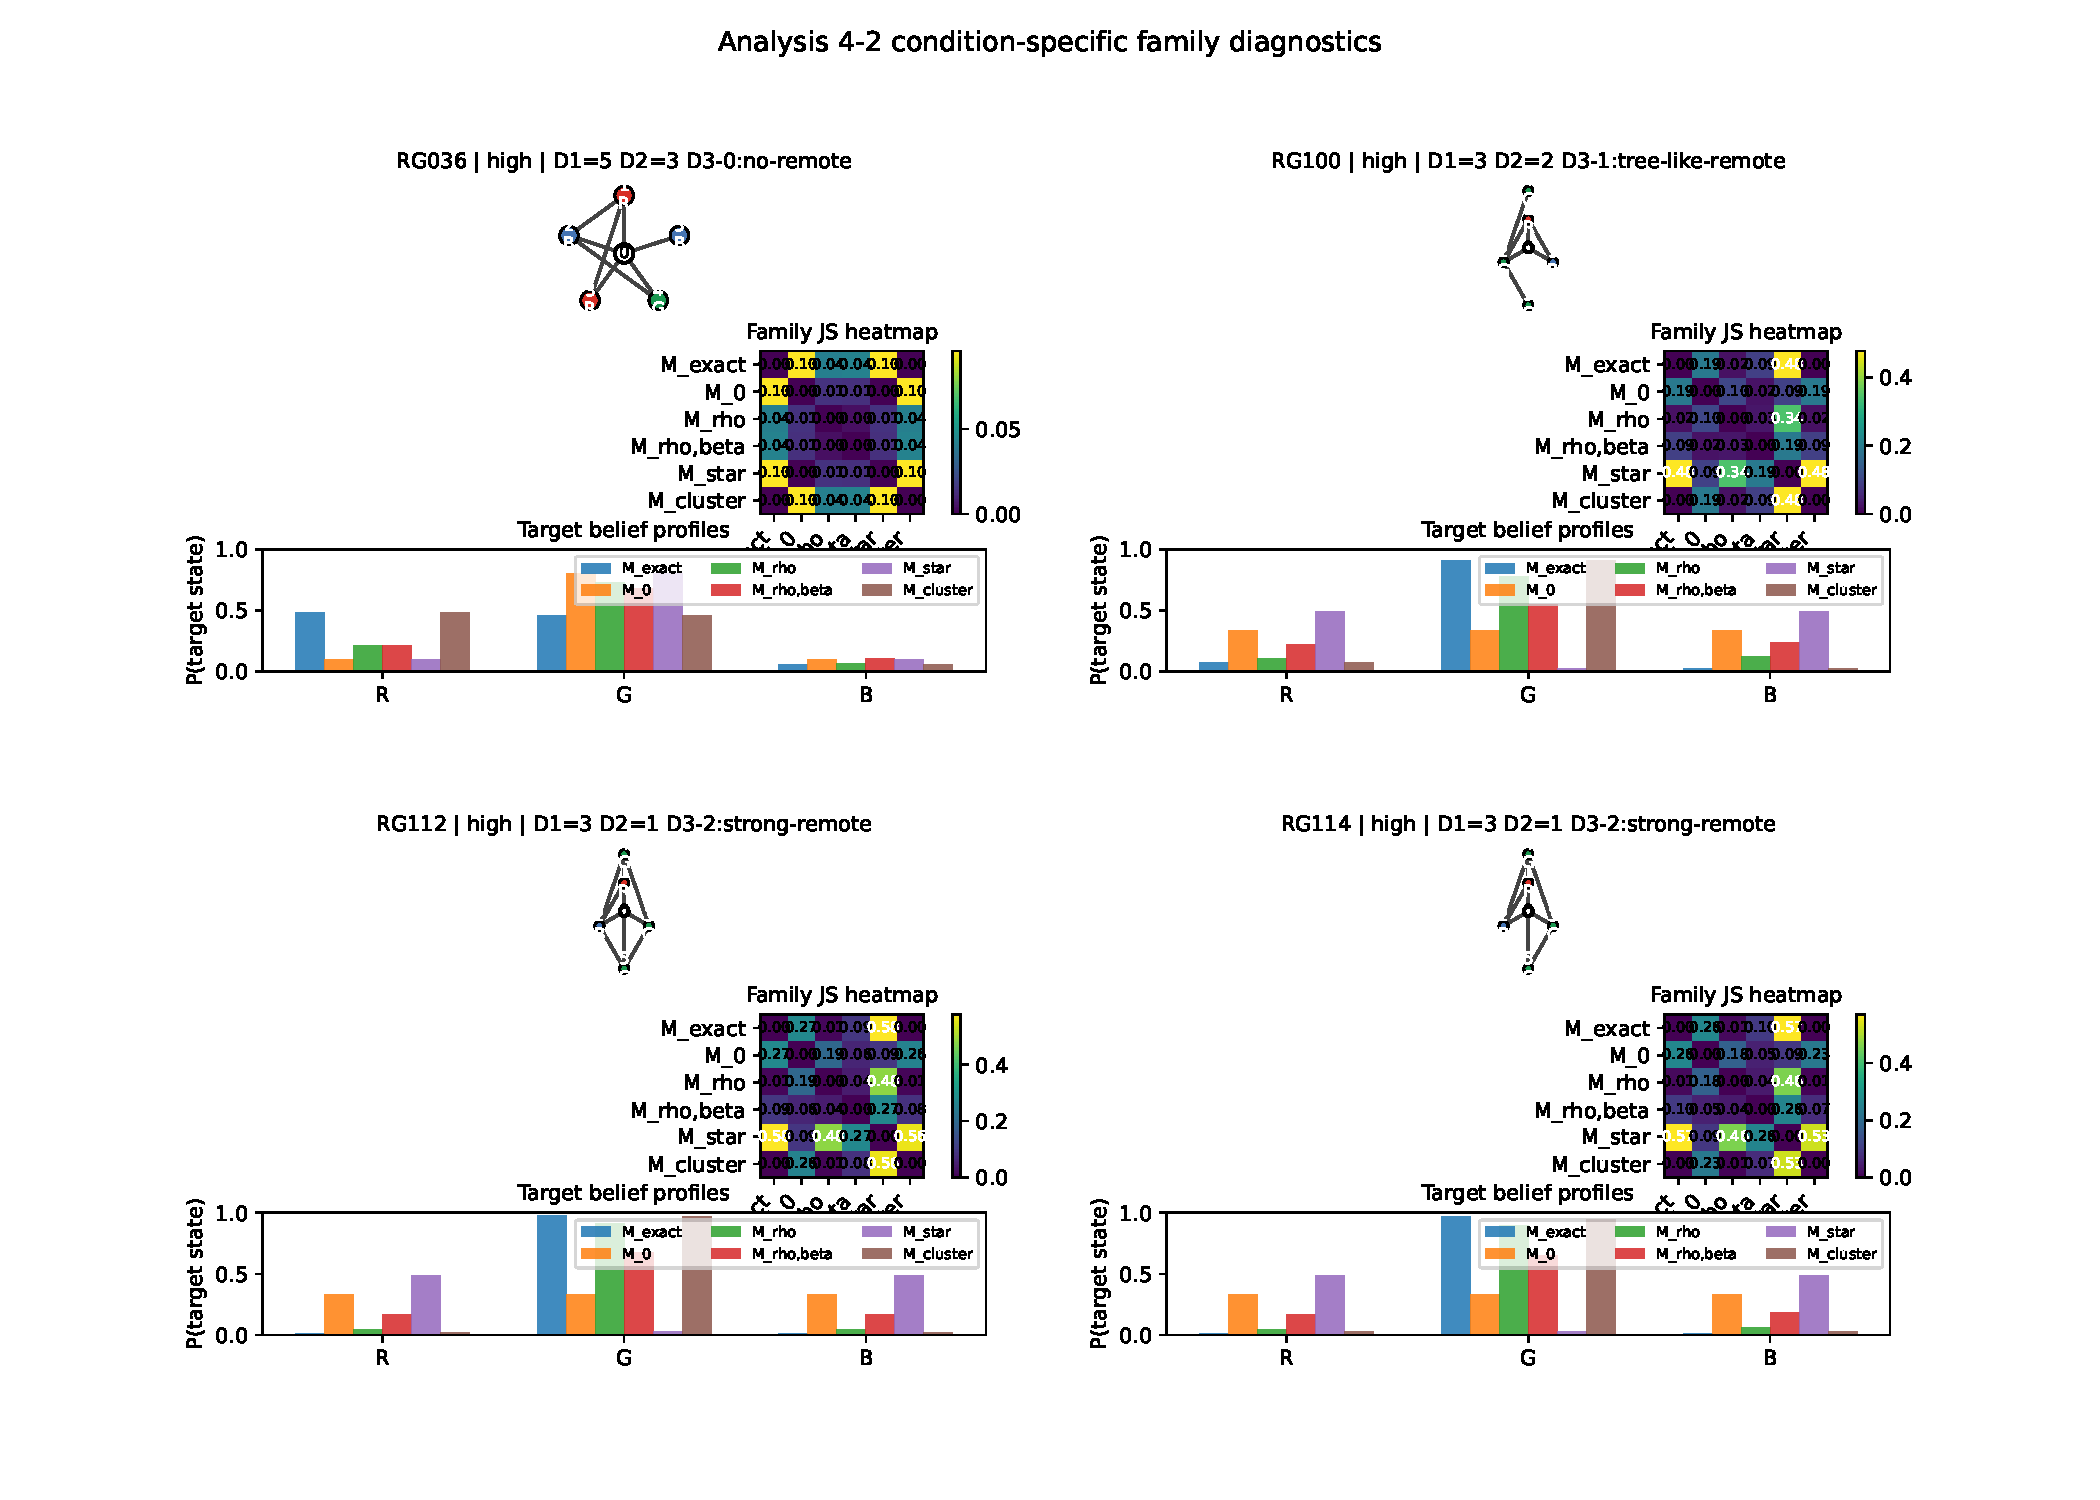
\includegraphics[width=\textwidth]{analysis-4-2_fig1_condition_panels.pdf}
\caption{Condition-specific family diagnostics for four representative rooted graph/evidence conditions.}
\end{figure}

\begin{figure}[H]
\centering
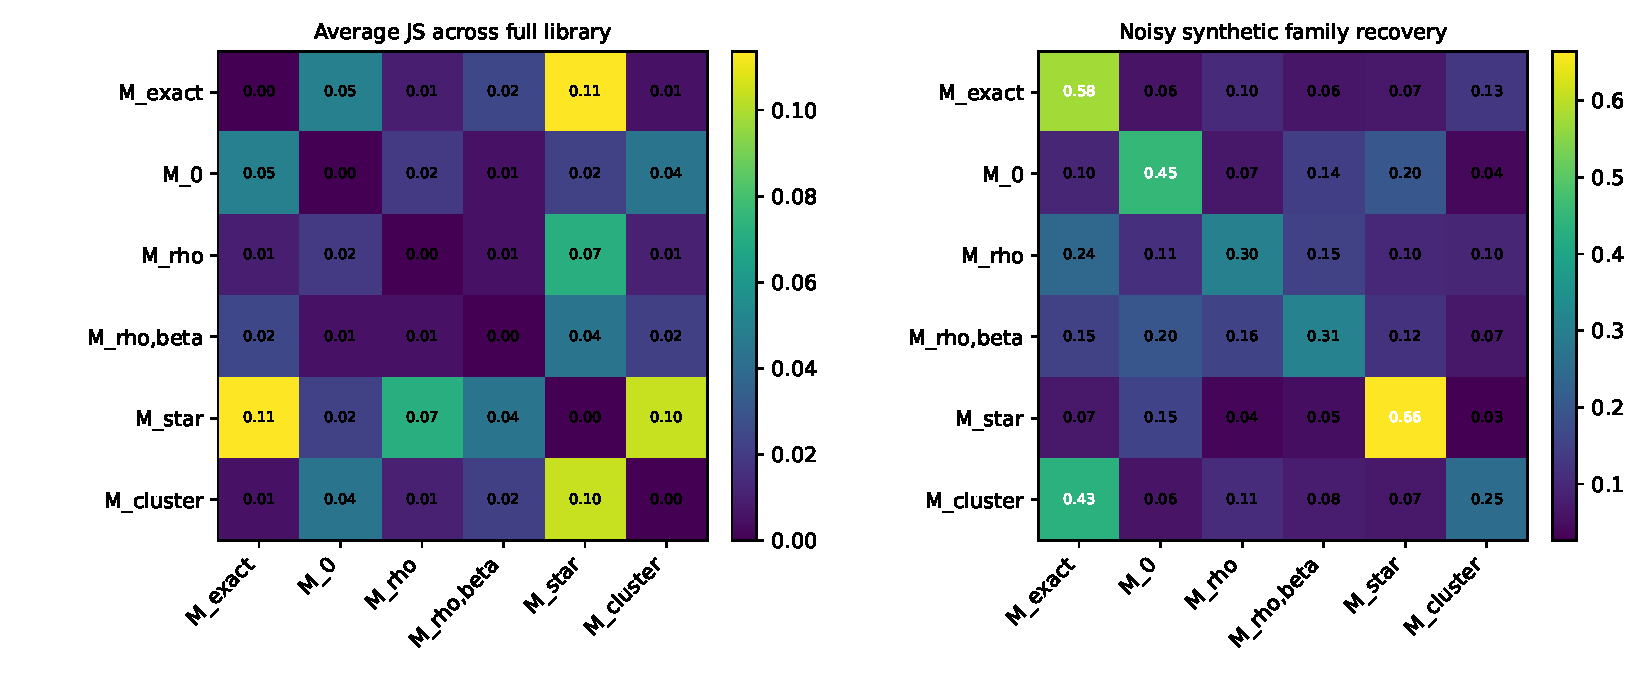
\includegraphics[width=0.9\textwidth]{analysis-4-2_fig2_global_confusion.pdf}
\caption{Global family confusion summary across the full rooted library.}
\end{figure}

\section{Conclusions against the TODO}
\begin{enumerate}
    \item The current rooted library already separates several cross-family comparisons strongly, especially those involving $M_{\mathrm{star}}$.
    \item D3-rich remote structure is particularly diagnostic for family-level contrasts.
    \item A compact reduced panel is now available for future behavioural use.
    \item Weak canonical separation between $M_{\rho}$ and $M_{\mathrm{exact}}$ motivates Analysis 4-3 and possibly richer task designs.
\end{enumerate}

\bibliographystyle{apalike}
\bibliography{../../manuscript/library}
\end{document}
